\documentclass{article}
\usepackage[margin=1in]{geometry}
\usepackage[outputdir=../]{minted}
\usepackage{graphicx}
\usepackage{booktabs}
\usepackage{siunitx}

\sisetup{
  round-mode = places,
  round-precision = 3,
  table-format = 1.3
}

\begin{document}

\title{CIS325: Classification for Bank Telemarketing Final}
\author{
  Christian Weber\\
  \texttt{christianweber2027@u.northwestern.edu}
}

\date{June 6th, 2025}
\maketitle


\section{Overview}

In this paper, we investigate the data surrounding, and build a model for a set of data representing the output of Bank Telemarketing campaigns. Our task is to understand if there is a common pattern in predicting the feature “y,” which has a classification of “Yes,” or “No.”

\section{Data Collection}

The data was collected by downloading from the Canvas website. It was then loaded into a Jupyter notebook for data cleaning, exploration and feature engineering.

\section{Data Cleaning}

The data was already sanitary with no null values or empty data missing.

\section{Feature Engineering}

The "Age" column spans a wide range of continuous values. The age column was used to create a new column of "Age Groups," a categorical feature that groups the age of the person represented in the row into an age bucket. For example, those under 17 are listed as youth. Those between 17-25 are listed as Adults. 25-60 are listed as Older Adults, and above 60 are listed as Seniors. The distribution of these buckets is shown below, with a large representation of older adults, those between the ages of 25 and 60.

\begin{figure}[H]
    \centering
    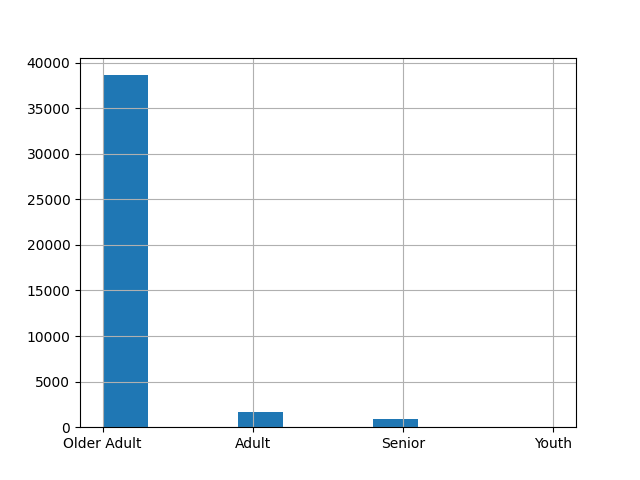
\includegraphics[width=0.75\linewidth]{paper/age_groups.png}
    \caption{Model and API Architecture}
    \label{fig:enter-label}
\end{figure}

\section{Data Normalization}

Every feature in the dataset was categorized as a Numerical, Categorical, or Ordinal Feature. Using scikit-learn, a Data Processing pipeline was used to convert the dataset into an efficient format for model training. Examples can be observed in the attached Jupyter Notebook.



\section{Determining most important features}

To determine the most important features, a RandomForest Classifier was used, pointing towards the target feature of "y." After preprocessing the data for normalization, the most important features were extracted and displayed in the table below. The top 3 features were then used for continued model experimentation as they had greater importance than the other features shown.

\begin{table}[htbp]
    \centering
    \caption{Feature Importance Rankings}
    \label{tab:feature_importance}
    \begin{tabular}{clS}
        \toprule
        \textbf{Rank} & \textbf{Feature} & \textbf{Importance} \\
        \midrule
        1 & duration                      & 0.266149 \\
        2 & euribor3m                     & 0.088633 \\
        3 & age                           & 0.080008 \\
        4 & nr.employed                   & 0.040371 \\
        5 & cons.conf.idx                 & 0.025803 \\
        6 & cons.price.idx                & 0.023981 \\
        7 & housing                       & 0.021655 \\
        8 & emp.var.rate                  & 0.021210 \\
        9 & pdays\_999                    & 0.020105 \\
        10 & poutcome\_success            & 0.019330 \\
        \bottomrule
    \end{tabular}
\end{table}

\section{Selecting the best model for training}

Cross validation was undertaken against a Logistic Regression, Support Vector Classifier, and a Random Forest Classifier. Hyperparameter tuning was also used to select the best hyperparameters for each model.

It was determined that the RandomForestClassifier in scikit-learn achieved 91\% accuracy on previously unseen testing data, after cross validation testing.

The model was then compiled with mlflow's save\_mmodel method as part of it's sklearn package. This was then stored in a directory where we could deploy the model as part of a great RESTful API web service.

\section{Deploying the Random Forest Classifier Model}
Next, we deployed the model using Flask and Python. Flask provides the ability to deploy a RESTful API onto a server. We created an endpoint to intake our most important feature's values as inputs, which then return a probability matrix against the target feature of y.

The model and application architecture is as follows:

\begin{figure}[H]
    \centering
    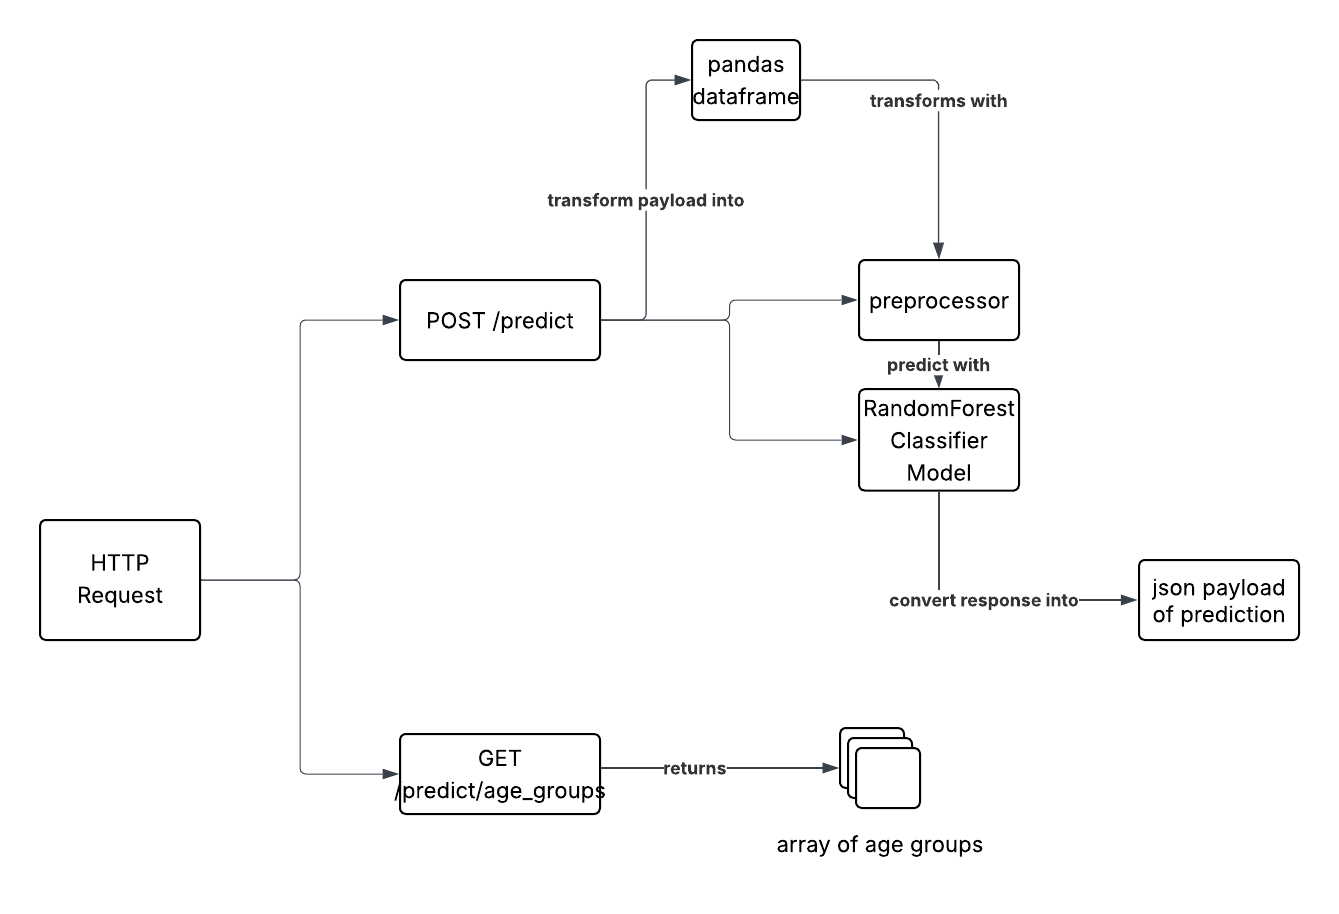
\includegraphics[width=0.75\linewidth]{paper/Code Layout-Final.png}
    \caption{Model and API Architecture}
    \label{fig:enter-label}
\end{figure}

As of publication, these endpoints are still live for testing:
\newline
\newline
http://ec2-3-94-179-40.compute-1.amazonaws.com/predict
\newline

To make a preodiction given our most important features, use curl:

\noindent\begin{minipage}{\linewidth}
\begin{minted}[fontsize=\footnotesize, breaklines, frame=single]{bash}
curl -X POST http://ec2-3-94-179-40.compute-1.amazonaws.com/predict \
-H "Content-Type: application/json" \
-d '{"duration": 120, "euribor3m": 6.00, "age_group": "Adult"}'

{"prediction":"N","probabilities":{"N":0.86,"Y":0.14}}
\end{minted}
\end{minipage}

All code can be found at https://github.com/webdog/cis325-final-part1

\section{Conclusion}

In conclusion, we built a Random Forest Classification model to predict feature "y," with existing features in the dataset of "duration" and "euribor3m." We then conducted feature engineering to create buckets of age groups to create categories of ages for the model to train against. This resulted in a Flask API application capable of taking inputs and producing probability outputs.

\section{License}
MIT License. Copyright (c) 2025 Christian Weber.

\end{document}